\documentclass[10pt, a4paper]{article}

%Preambuła dokumentu
\usepackage{graphicx}       % pakiet graficzny, umożliwiający m.in.
                            % import grafik w formacie eps
\usepackage{rotating}       % pakiet umożliwiający obracanie rysunków
\usepackage{subfigure}      % pakiet umożliwiający tworzenie podrysunków
\usepackage{epic}           % pakiet umożliwiający rysowanie w środowisku latex
\usepackage{listings}       % pakiet dedykowany zrodlom programow
\usepackage{verbatim}       % pakiet dedykowany rozmaitym wydrukom tekstowym
\usepackage{amssymb}        % pakiet z rozmaitymi symbolami matematycznymi
\usepackage{amsmath}        % pakiet z rozmaitymi środowiskami matematycznymi
\usepackage[polish]{babel}  % pakiet lokalizujący dokument w języku polskim
\usepackage[OT4]{fontenc}
\usepackage[utf8]{inputenc} % w miejsce utf8 można wpisać latin2 bądź cp1250,
                            % w zależności od tego w jaki sposób kodowane są 
                            % polskie znaki diakrytyczne przy wprowadzaniu 
                            % z klawiatury.

\usepackage[draft]{prelim2e}% informacja w stopcje o statusie dokumentu 
                            % (draft-szkic lub final-wersja ostateczna) 

\textwidth      16cm
\textheight     25.5cm
\evensidemargin -3mm
\oddsidemargin  -3mm
\topmargin      -20mm


% deklaracje wymagane przez funkcję drukującą tytuł dokumentu:
%
\author{Automatyka i Robotyka, specjalność Robotyka\footnote{Wydział Elektroniki, Politechnika Wrocławska, ul. Z. Janiszewskiego 11/17, 50-372 Wrocław} }

 
\title{ Wirtualne laboratorium robotyki - Instrukcja } 

\date{\today}

% Koniec preambuły dokumentu

% Tekst dokumentu

\begin{document}
\maketitle % drukuje tytul, autora i datę zdefiniowaną w preambule
%
%\the\setitem
\def\tablename{Tabela}
%

\section{Wstęp}
\label{sec:wstep} % definicja etykiety rozdziału
W niniejszej instrukcji znajduje się opis czynności potrzebnych do uruchomienia i użytkowania systemu wirtualnego laboratorium.

\section{Przygotowanie systemu do uruchomienia}
\label{sec:przygotowanie}
Do uruchomiania systemu wymagane jest zainstalowanie lokalnie Dockera. W przypadku braku tego pakietu na komputerze należy postąpić zgodnie z instrukcją zamieszoną na stronie Dockera:

\begin{verbatim}
https://docs.docker.com/engine/installation/linux/ubuntu/
\end{verbatim}


Aby nie musieć za każdym razem używać $sudo$ w poleceniach dotyczących Dockera należy po zakończeniu instalacji wykonać polecenie:
\begin{verbatim}
 sudo usermod -aG docker [nazwa twojego użytkownika] 
\end{verbatim}

i potwierdzić hasłem użytkownika. 

Następnie należy pobrać na dysk lokalny obraz systemu znajdujący się w repozytorium DockerHub. Należy pobrać najnowszy obraz wersji beta o nazwie :
\begin{verbatim}
 projektprzejsciowy2016$/docker_lab_beta:latest
\end{verbatim}

Możliwe jest to za pomocą polecenia:
\begin{verbatim}
docker pull projektprzejsciowy2016/docker_lab_beta:latest
\end{verbatim}


\begin{figure}[hbt]
  \setlength{\unitlength}{1.0cm}
  \centering 
  
    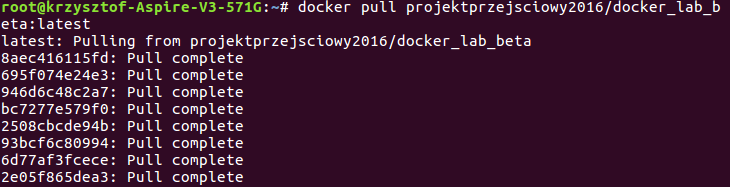
\includegraphics[width=12 cm]{./grafika/pull.png}
 
\end{figure}


Przed uruchomieniem obrazu należy zezwolić wszystkim aplikacjom działającym z poziomu Dockera na uruchamianie się w trybie graficznym:
\begin{verbatim}
 xhost +
\end{verbatim}

Powinien pojawić się następujący komunikat:
$"$access control disabled, clients can connect from any host$"$

Uruchomienie obrazu systemu odbywa się poprzez wpisanie w konsoli polecenia (powoduje stworzenie nowego kontenera, na podstawie wywołanego i otwiera go - wszelkie zmiany będą zapisywane w nowym kontenerze) :

\begin{verbatim}
 docker run -it -e DISPLAY=unix$DISPLAY -v=/tmp/.X11-unix:/tmp/.X11-unix:rw \
 projektprzejsciowy2016/docker_lab_beta:latest

\end{verbatim}

W przypadku gdy potrzebujemy współdzielić pewne katalogi lokalne z Dockerem należy  w poleceniu uruchamiającym obraz systemu $"$docker run$"$ skorzystać z opcji -v:
\begin{verbatim}
docker run -it -e DISPLAY=unix$DISPLAY -v=/tmp/.X11-unix:/tmp/.X11-unix:rw \
-v[scieżka_do_katalogu_lokalnego]:[scieżka_gdzie_ma_być_montowany_w_obrazie] \
projektprzejsciowy2016/docker_lab_beta:latest

\end{verbatim}


System ROS wraz z symulatorem - Gazebo, uruchamiany jest poleceniem wykonywanym już z poziomu obrazu Dockera:
\begin{verbatim}
roslaunch projekt_przejsciowy l15.launch &
\end{verbatim} 

Po chwili powinien uruchomić się symulator Gazebo:

\begin{figure}[hbt]
  \setlength{\unitlength}{1.0cm}
  \centering 
  
    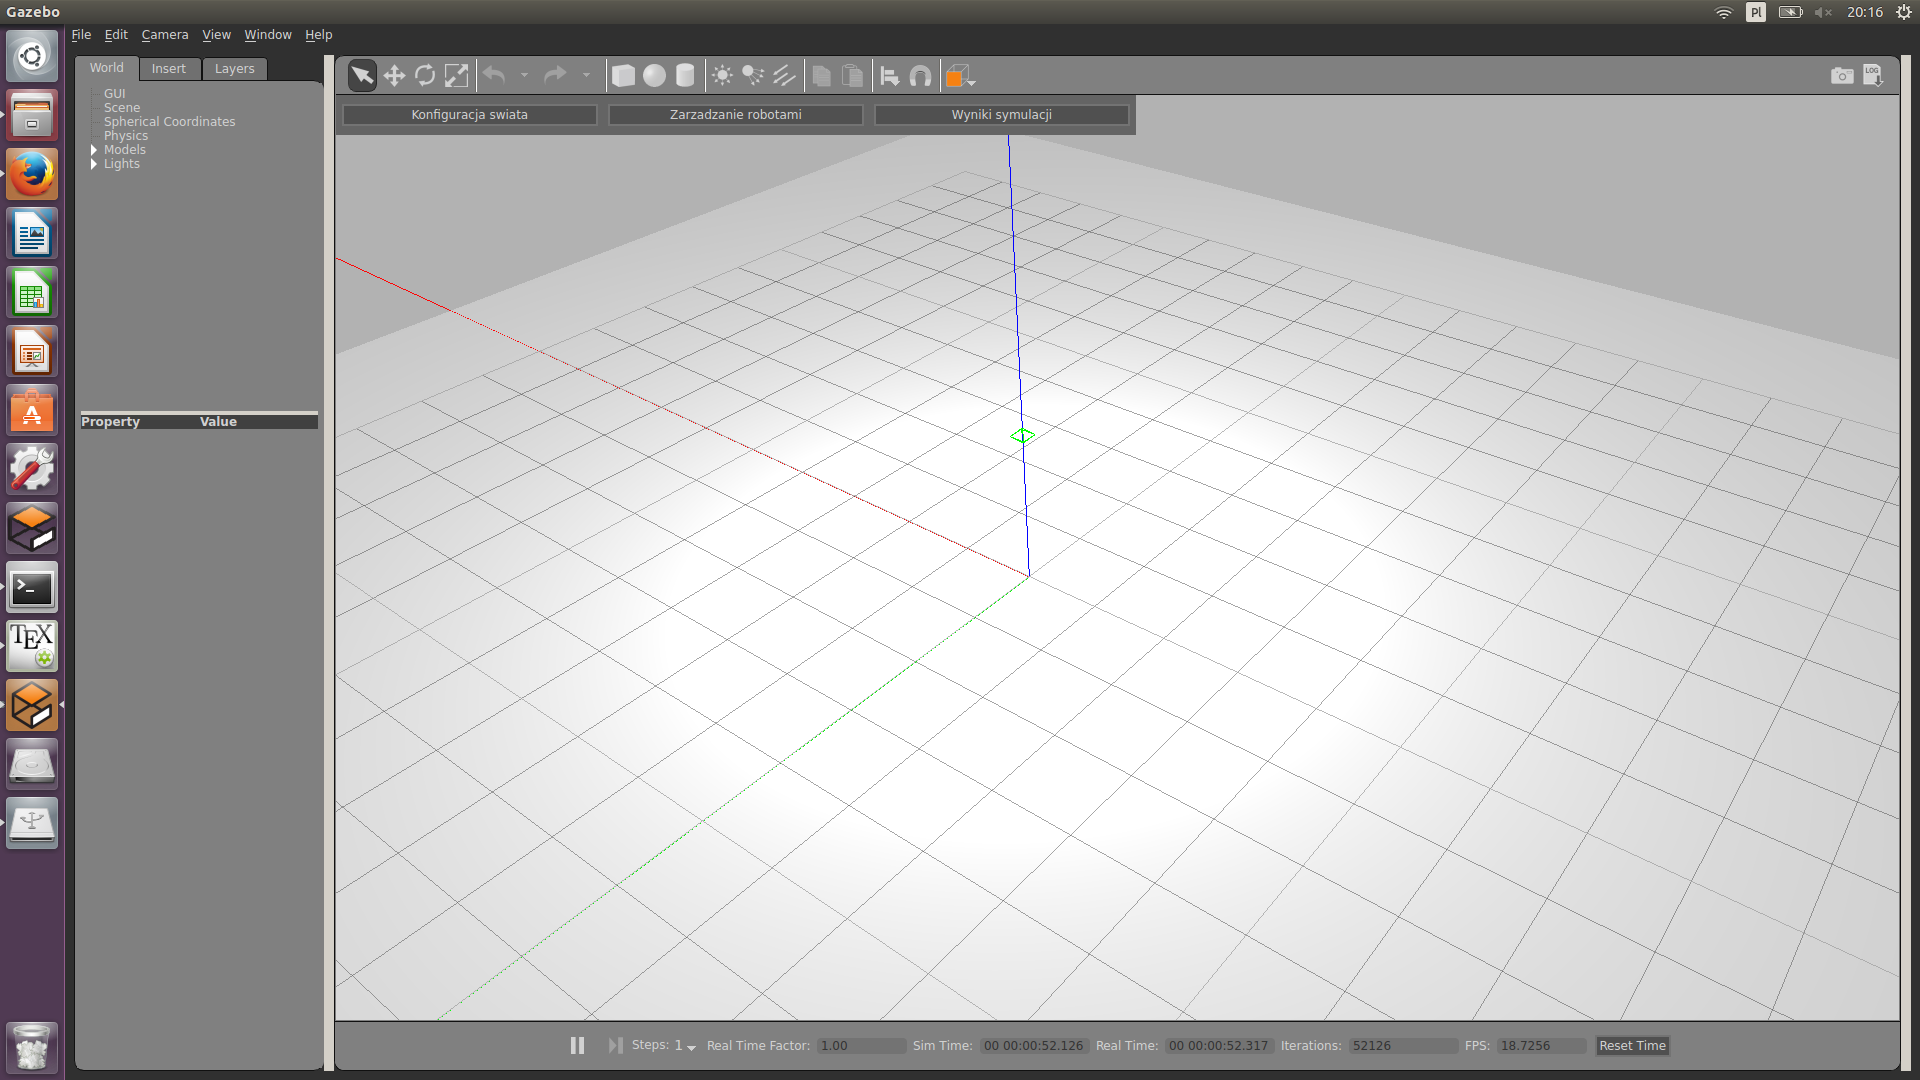
\includegraphics[width=12 cm]{./grafika/EkranGlowny.png}

\end{figure}
 Aby przetestować czy wszystko działa poprawnie należy dodać na scenę robota jak w puncie 3.2.


Jeśli potrzebujemy uruchomić drugą konsolę działającą na tym samym kontenerze to należy uruchomić drugą konsolę (można to wykonać skrótem klawiszowym $"$shitf$"$+$"$ctrl$"$+$"$t$"$, a następnie sprawdzamy nazwę kontenera, który mamy już uruchomiony:

 \begin{verbatim}
docker ps -a
\end{verbatim}


Powyższe polecenia wyświetla listę wszystkich dostępnych lokalnie kontenerów, w której można sprawdzić nazwy poszczególnych kontenerów:


\begin{figure}[hbt]
  \setlength{\unitlength}{1.0cm}
  \centering 
  
    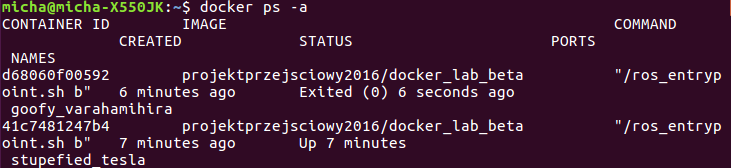
\includegraphics[width=12 cm]{./grafika/ps-a.png}

\end{figure}

Na przedstawionej na rysunku liście przykładowe nazwy to goofy\_varahamihira oraz stupefied\_tesla. Podpięcie się konsolą pod otwarty już kontener opiera się o polecenie:


 \begin{verbatim}
docker exec -it Nazwa_Kontenera bash
\end{verbatim}


Uruchamiając kontener po raz kolejny mamy możliwość zachowania historii wykorzystywanych poleceń. Przy uruchamianiu kontenera odwołujemy się do ostatniego otwieranego dockera:
\begin{verbatim}
docker start -i $(docker ps -q -l)
\end{verbatim}



\section{Obsługa systemu}
\subsection{Dodawanie modelu sali}
Na obrazie systemu, w chwili obecnej, znajdują się trzy przykładowe modele świata:
\begin{itemize}
\item model sali L1.5 w budynku C-16
\item dwa dodatkowe modele składające się z ułożonych w pewien sposób mebli 
\end{itemize}

Dodanie jednego z tych światów możliwe jest z poziomu okna "Konfiguracja Świata". Dostep do wspomnianego okna jest z poziomu widoku głównego Gazebo pod przyciskiem umieszczonym z lewej strony listwy na górze ekranu.
\begin{figure}[hbt]
  \setlength{\unitlength}{1.0cm}
  \centering 
  
    \includegraphics[width=12 cm]{./grafika/KOnfiguracjaSwiata.png}

\end{figure}
W oknie tym, po lewej stronie, znajduje się lista dostępnych światów oraz dwa przyciski "Wczytaj" i "Wyczyść". Wybraną salę można dodać wybierając ją z lisy i klikając pierwszy przycisk. Jeśli wczytamy inną salę w momencie, gdy jakaś jest już wczytana, scena zostanie automatycznie wyczyszczona i wczytany aktualnie wybrany świat. Przycisk "Wyczyść$"$ służy do usunięcia wszystkich obiektów ze sceny z wyjątkiem robotów.

 \subsection{Dodawanie modeli robotów}
Z okna konfiguracji świata można również dodawać na scenę roboty (jak narazie dostępne są trzy roboty Pioneer). Służą do tego listy na środku oraz z prawej strony okienka. Lista środkowa zawiera roboty, które są dostępne do dodania, a prawa te, które są już dodane. Aby dodać robota, należy wybrać go z listy środkowej i kliknąć przycisk " Dodaj". Roboty dodane pojawią się na scenie w momencie kliknięcia przycisku $"$Zatwierdź$"$.  W tym samym momencie pojawiają się w systemie ROS topiki związane z dodawanymi robotami. Listę topików można zobaczyć wpisując w terminalu:
\begin{verbatim}
rostopic list
\end{verbatim}
Przycisk $"$Schowaj" umieszcza wybranego robota poza salą w tak zwanym schowku.

Aby przetestować czy Gazebo dobrze współpracuje z systemem ROS należy dodać robota a następnie w konsoli wydać polecenie publikujące w topicu ROSa odpowiadającym za prędkość dodanego robota:
\begin{verbatim}
rostopic  pub /pionner_1/RosAria/cmd_vel geometry_msgs/Twist \
-- '[1.0, 0.0, 0.0]' '[0.0, 0.0, -0.5]
\end{verbatim}

W efekcie robot powinien zacząć poruszać się po okręgu.

\begin{figure}[hbt]
  \setlength{\unitlength}{1.0cm}
  \centering 
  
    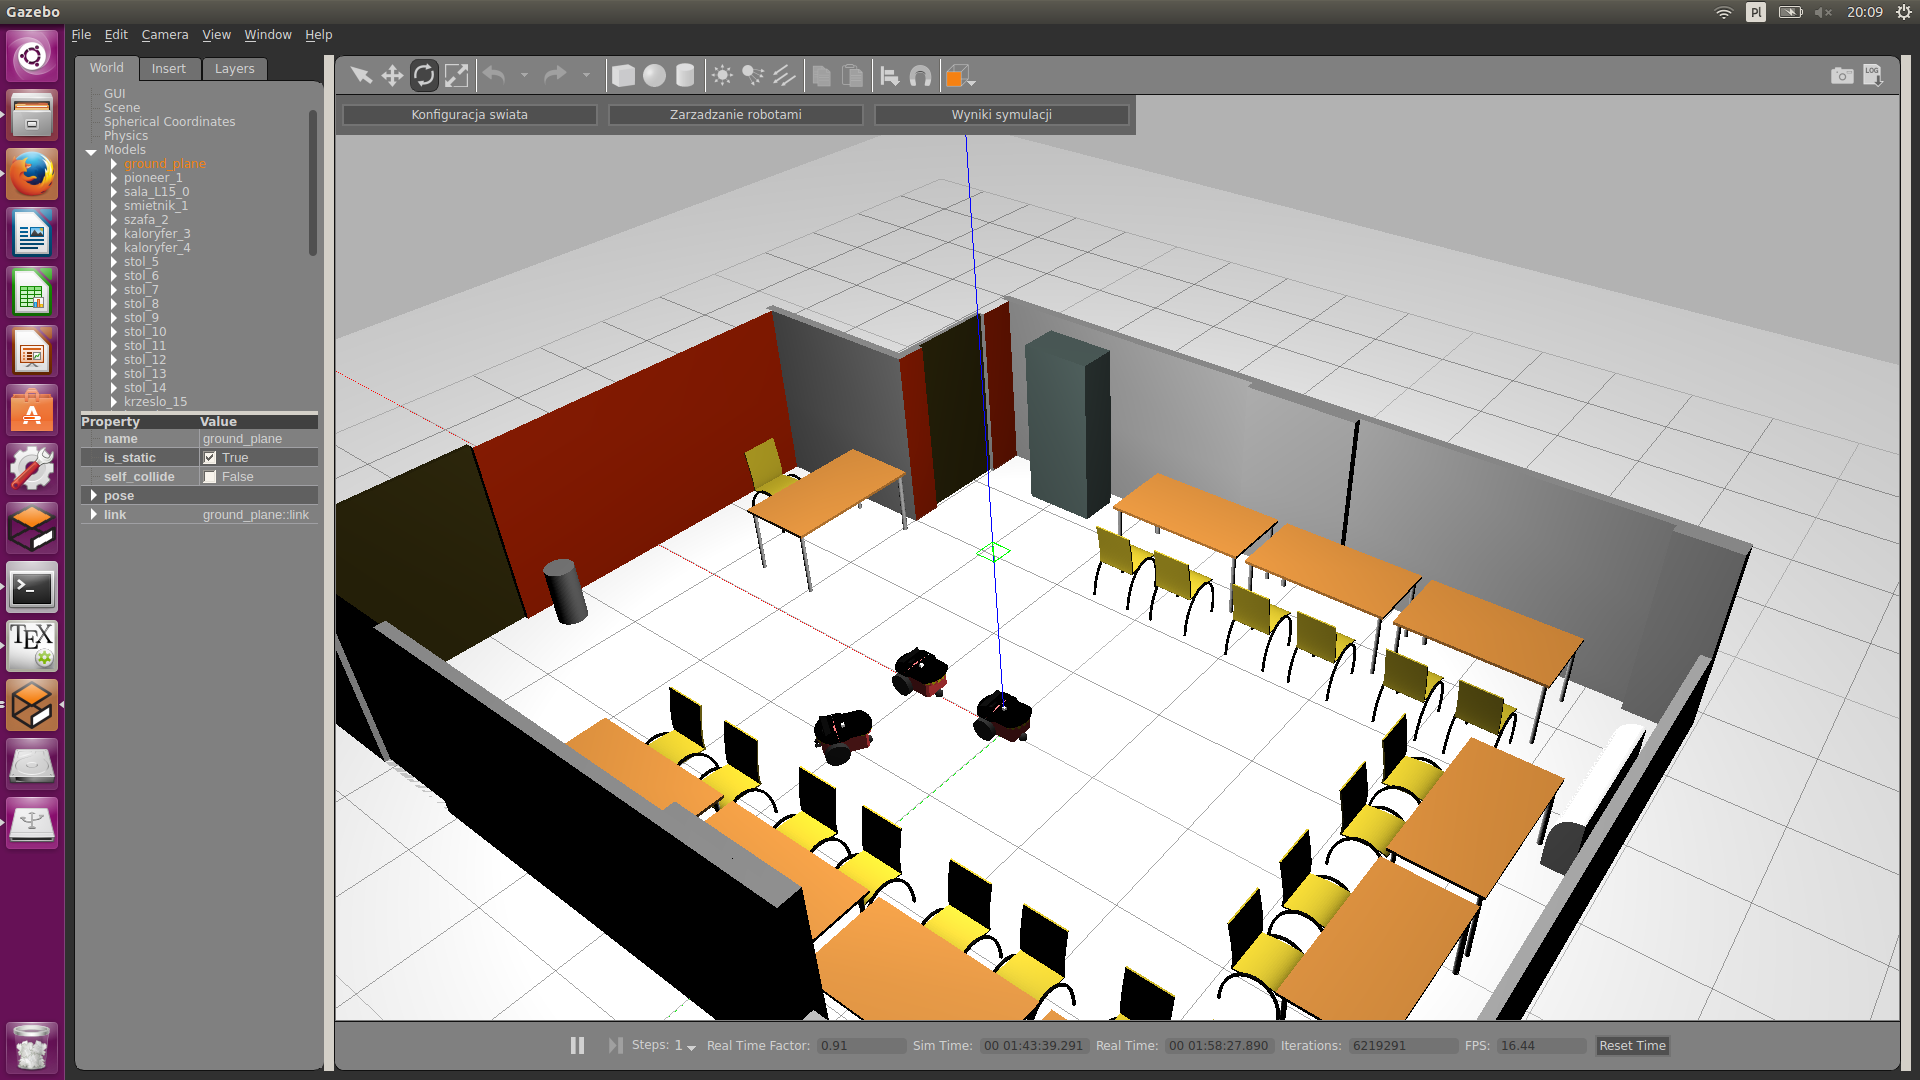
\includegraphics[width=12 cm]{./grafika/EkranGlownyZSalaIRobotami.png}

\end{figure}

 \subsection{Resetowanie robotów i ustawianie ich w zadanych miejscach}

Do resetowania i ustawiania w zadanej pozycji robotów służy okno $"$Zarządzanie robotami". Okno podzielone jest na zakładki - każda z nich dotyczy osobnego robota. Umieszczony w każdej zakładce przycisk $"$Reset$"$ ustawia odpowiedniego robota w punkcie (0,0) sali z orientacją równą 0. Pola tekstowe służą do zadawania pozycji (X,Y) i orientacji robota. Wartości z tych pól są wykorzystywane przy używaniu przycisku "Ustaw". W trakcie kliknięcia wartości te są sprawdzane i ich ewentualna niepoprawność jest sygnalizowana czerwonym podświetleniem pola. Dopiero po sprawdzeniu robot przemieszczany jest na ustaloną pozycję.
\begin{figure}[hbt]
  \setlength{\unitlength}{1.0cm}
  \centering 
  
    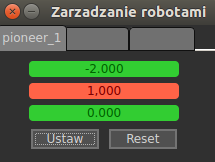
\includegraphics[width=6 cm]{./grafika/OknoZarzadzaniaRobotami.png}

\end{figure}


\subsection{Wyświetlanie i zapisywanie wyników}
Do wizualizacji i zapisu danych z eksperymentu przygotowane zostało okno $"$Wyniki symulacji$"$. Okno podzielone jest na zakładki, w których można otrzymać podgląd trajektorii wszystkich robotów oraz przebiegi położenia X, Y i orientacji. W pierwszej zakładce są trasy przebyte przez wszystkie roboty a każda kolejna zakładka odnosi się do konkretnego robota prezentując jego położenie i orientację. Przycisk $"$Reset danych$"$ pozwala wyczyścić wykresy i zacząć zbierać je od nowa.  Okno daje możliwość zapisania przebiegów do plików, które znajdują się potem w folderze /root/.  Ważne jest też aby przed rozpoczęciem zbierania danych do konkretnego wykresu za pomocą przycisku z dolnego paska Gazebo $"$PLAY/PAUSE$"$ zatrzymać czas symulacyjny następnie przyciskiem $"$Reset Time$"$ aby wykres był czytelny.
\begin{figure}[hbt]
  \setlength{\unitlength}{1.0cm}
  \centering 
  
    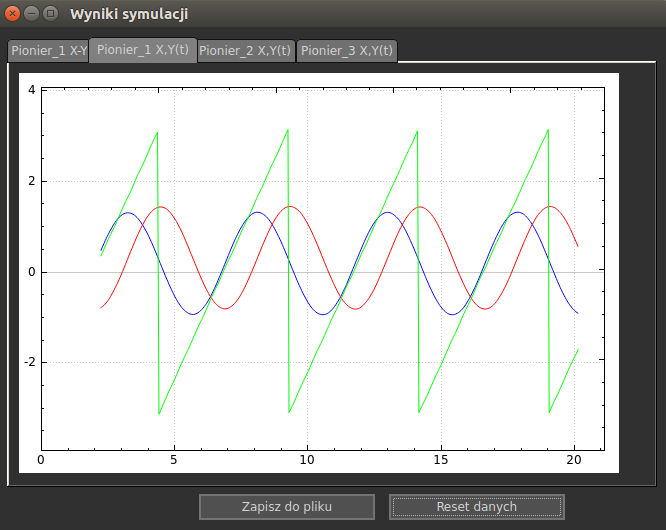
\includegraphics[width=6 cm]{./grafika/Wykres.png}

\end{figure}

\subsection{Wyświetlanie odczytów z czujników}
Aby uzyskać dostęp do pomiarów z czujników należy z paska narzędzi Gazebo wybrać zakładkę $Window$ $>>$ $Topic$ $Visualization$. Uruchomi się okno:
 \begin{figure}[hbt]
  \setlength{\unitlength}{1.0cm}
  \centering 
  
    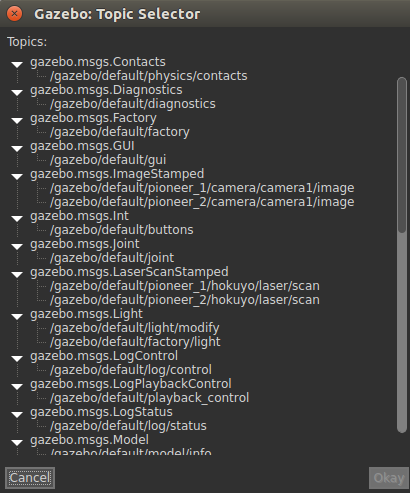
\includegraphics[width=6 cm]{./grafika/WizualizacjaLista.png}

\end{figure}

Następnie wybieramy topic czujnika, z którego chcemy wyświetlać dane. Dla skanera laserowego wykres wygląda następująco:

 \begin{figure}[hbt]
  \setlength{\unitlength}{1.0cm}
  \centering 
  
    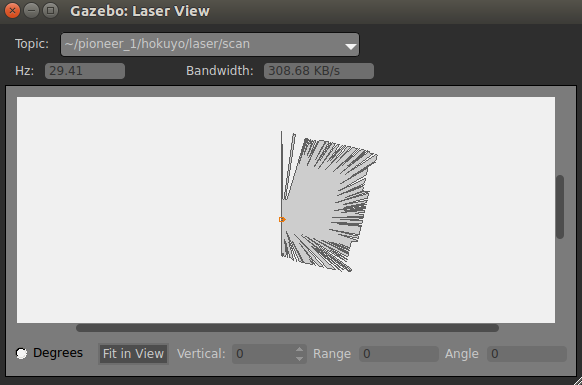
\includegraphics[width=8 cm]{./grafika/Skaner.png}

\end{figure}
\newpage
\subsection{Dodawanie i edycja modeli przeszkód na scenie}
Aby dodać przeszkodę na scenę należy z lewej strony ekranu wejść w zakładkę "Insert", wybrać kliknięciem model i kliknąć na miejsce na scenie, w którym chcemy postawić przeszkodę. Proste modele przeszkód dostępne są z paska narzędzi Gazabo. 
Aby zmienić statyczność przeszkody należy kliknąć na nią prawym przyciskiem myszy (PPM) a następnie z rozwiniętego menu wybrać opcję $"$Edit Model". Gazebo przejdzie do trybu edycji modelu. Wybieramy zakładkę "Model" i zaznaczamy lub odznaczamy opcję $"$Static":

\begin{figure}[hbt]
  \setlength{\unitlength}{1.0cm}
  \centering 
  
    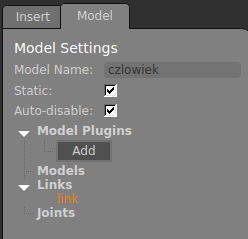
\includegraphics[width=6 cm]{./grafika/Edit.png}

\end{figure}



\end{document}
 
